%%%%%%%%%%%%%%%%%%%%%%%%%%%%%%%%%%%%%%%%%%%%%%%%%%%%%%%%%%%%%%%%%%%%%%%%%%%%%%%%%%%%%%%%%%%%%%%%%%%%%%%%%%%%%%%%%%%%
%%%%%%%%%%%%%%%%%%%%%%%%%%%%%%%%%%%%%%%%%%%%%%%%%%%%%%%%%%%%%%%%%%%%%%%%%%%%%%%%%%%%%%%%%%%%%%%%%%%%%%%%%%%%%%%%%%%%
\section{Introdução}

É com grande felicidade que oferecemos este texto modelo para o \textit{short paper} (2--6 páginas) para o VI Seminário Gaúcho de Acústica e Vibrações (edição \textit{e-letrônica}, em 2021). Serão aceitos apenas \textit{short papers} de trabalhos inéditos. Trabalhos já publicados também podem ser apresentados no VI~SeGAV-e, desde que título, resumo original e evento original (ou revista) sejam evidenciados de acordo (na submissão do resumo).
%
Observe o diagrama da \figura{fig:reusmao}, que contém um sumário de datas e direções do evento.

Este texto de instruções foi elaborado para que os autores possam apresentar os artigos de forma padronizada, ele foi adaptado do modelo de artigo da Revista Acústica \& Vibrações \cite{modelo}. Isso facilitará muito o trabalho de revisão e diagramação, proporcionando uma uniformidade de texto para os artigos. Neste modelo são apresentadas as principais diretrizes para a elaboração do artigo completo no que diz respeito à apresentação de conteúdo, gráfica, estrutura e ao procedimento para a submissão dos artigos.
% 
Este documento já possui a formatação de estilos personalizados para a elaboração do texto. O autor pode, portanto, utilizar este arquivo como modelo para esta finalidade. Serão disponibilizados modelos (\textit{templates}) em Microsoft Word (.docx) e \LaTeX\xspace (.tex). Esta versão também está disponível no \href{https://www.overleaf.com/read/gtxwpfrgdtgk}{Overleaf}. Os autores são responsáveis por enviar os artigos de acordo com o modelo vigente do evento.

O texto completo deverá estar em espaçamento simples entre linhas, tipografia (fonte) Palatino Linotype (ou Times New Roman) tamanho 12~pt e parágrafo com espaçamento de 0~pt antes e 8~pt depois. É prática comum a escrita de artigos científicos no impessoal, logo, recomenda-se essa prática. Além disso, serão aceitos em língua culta portuguesa, inglesa\footnote{Artigos em língua estrangeira deverão passar por correção profissional de língua. Em inglês, o revisor profissional Joseph Lacey (\href{mailto:joe.traduz@gmail.com}{joe.traduz@gmail.com}), americano nativo, é o conveniado do SeGAV.} e espanhola. 

\begin{figure}[ht!]
	\centering 
        
\includegraphics[width=0.98\linewidth,page=3]{segav.pdf}
        \caption{Resumo de etapas do VI SeGAV-e 2021. Link para inscrição de participante direto no YouTube e link para inscrever resumo \url{https://forms.gle/9KvUSk6T136cN2DU8}.}
	\label{fig:reusmao}%
\end{figure}

%%%%%%%%%%%%%%%%%%%%%%%%%%%%%%%%%%%%%%%%%%%%%%%%%%%%%%%%%%%%%%%%%%%%%%%%%%%%%%%%%%%%%%%%%%%%%%%%%%%%%%%%%%%%%%%%%%%
%%%%%%%%%%%%%%%%%%%%%%%%%%%%%%%%%%%%%%%%%%%%%%%%%%%%%%%%%%%%%%%%%%%%%%%%%%%%%%%%%%%%%%%%%%%%%%%%%%%%%%%%%%%%%%%%%%%
\section{Orientações básicas}

Nesta seção há um resumo de como o artigo deve ser construído. Para mais detalhes, consulte as seções subsequentes.

%\vspace{-8pt}
\begin{enumerate} \itemsep=2pt
    \item Os modelos em LaTeX e Word fornecidos já contêm todas as configurações descritas neste documento. Além disso, este texto fornece simultaneamente instruções para as duas plataformas de diagramação de texto.
	\item A primeira página deve conter (para língua portuguesa) título, autores, filiações, resumo e palavras-chave. São opcionais \textit{title}, \textit{abstract} e \textit{keywords}, desde que não adentrem a segunda página do artigo.
	Submissões em espanhol devem ter itens similares, porém em língua espanhola. Submissões em inglês podem conter apenas \textit{title}, \textit{abstract} e \textit{keywords}.
	\item O texto deve ser escrito em língua culta vigente.
	\item \textbf{O número máximo de páginas é 6, contando da página que contém o título, até o final das referências.}
	\item O tamanho do papel é A4, com margens: superior de 2,0~cm, inferior de 2,0~cm, esquerda de 1,8~cm e direita de 1,8~cm (o espaçamento entre colunas é de 1,0~cm).
	\item O texto deve ser escrito com tipografia\linebreak Times New Roman ou Palatino Linotype com tamanho 12~pt (conforme este modelo).
	\item O artigo pode conter figuras, tabelas, quadros, códigos e equações. No texto, caso sejam necessários, links podem ser colocados. Animações também são aceitas, desde que estejam diagramadas como figuras.
	\item Entende-se que um artigo técnico tenha uma estrutura lógica, descritiva e conteúdo passível de reprodução, findando nas referências do trabalho.
\end{enumerate}


%%%%%%%%%%%%%%%%%%%%%%%%%%%%%%%%%%%%%%%%%%%%%%%%%%%%%%%%%%%%%%%%%%%%%%%%%%%%%%%%%%%%%%%%%%%%%%%%%%%%%%%%%%%%%%%%%%%%
%%%%%%%%%%%%%%%%%%%%%%%%%%%%%%%%%%%%%%%%%%%%%%%%%%%%%%%%%%%%%%%%%%%%%%%%%%%%%%%%%%%%%%%%%%%%%%%%%%%%%%%%%%%%%%%%%%%%
\section{Documento e apresentação}

Sempre coloque texto em seções e subseções, não as deixe órfãs (abrindo uma seção e passando direto para a subseção).

%%%%%%%%%%%%%%%%%%%%%%%%%%%%%%%%%%%%%%%%%%%%%%%%%%%%%%%%%%%%%%%%%%%%%%%%%%%%%%%%%%%%%%%%%%%%%%%%%%%%%%%%
\subsection{Primeira página}

A primeira página deve conter os seguintes itens colocados pelos autores: título, autores, filiações, resumo e palavras-chave. 
%
Caso o título completo seja muito extenso, pede-se uma versão curta para que seja incluída no cabeçalho das páginas do artigo. 

O resumo do artigo poderá ter entre 200 e 350 palavras. O título, resumo e palavras-chave constituem parte da primeira página do artigo. Ele deve fazer uma apresentação concisa do artigo técnico científico, contendo uma introdução, o objetivo, uma síntese da metodologia, o principal resultado e a principal conclusão (preferencialmente nessa ordem). Assim, o leitor pode conhecer a essência do conteúdo do artigo. Lembre-se que o resumo é como o \textit{trailer} de um filme, as pessoas ficarão interessadas em ler completamente o artigo se o resumo lhes interessar. O resumo não deve conter informações novas não contidas no artigo; abreviações indefinidas; discussão prévia de outra literatura; referências e citações e excesso de detalhes acerca dos métodos empregados. Ele também não é o parágrafo de introdução do documento, isso deve ser colocado no início do texto. Utilize apenas informações úteis e relevantes, faça um exercício de empatia com o possível leitor interessado. Para se obter um resumo coeso, elegante e de acordo com o artigo, escreva uma prévia, realize a escrita completa do documento e, ao final, revise-o observando se o conteúdo dele reflete de forma consistente o teor do documento. 

Seguindo o resumo, o autor deve listar até cinco palavras chaves (evite colocar as mesmas palavras que formam o título do artigo).

Na filiação dos autores use números como marcas e caso existam autores de uma mesma instituição, utilize apenas um endereço e os diferencie nos e-mails. Quando existirem e-mails de um mesmo domínio, busque reduzir usando chaves \{$\cdot$\}. Utilize no máximo duas linhas para a filiação de cada autor de instituições diferentes. Preste atenção nos exemplos:

\begin{flushleft}
%\vspace{-0.2\baselineskip}
\begin{itemize}[noitemsep,topsep=-1ex,align=left,leftmargin=0.2cm] \itemsep=10pt

	\item Fonseca,~W.~D'A.$^1$; Sobrenome,~N.$^2$\\[5pt]	
{\small		$^{1,2}$\,Engenharia Acústica, Universidade Federal de Santa Maria, Santa Maria, RS,\linebreak 
	 will.fonseca@eac.ufsm.br, nome@dominio.br.}
	
	\vspace{2mm}
	\item Fonseca,~W.~D'A.$^1$; Mareze,~P.~H.$^2$\\[5pt]	
{\small	$^{1-2}$\,Engenharia Acústica, Universidade Federal de Santa Maria, Santa Maria, RS, 
	\{will.fonseca, paulo.mareze\}@eac.ufsm.br.}
	
	\newpage
	
	\item Fonseca,~W.~D'A.$^1$; Sobrenome,~N.$^2$, Mareze,~P.~H.$^3$\\[6pt]	
{\small		$^{1,3,2}$\,Engenharia Acústica, Universidade Federal de Santa Maria, Santa Maria, RS, 
	\{will.fonseca, paulo.mareze\}@eac.ufsm.br,\linebreak nome@dominio.br.}

	\item Fonseca,~W.~D'A.$^1$; Sobrenome,~N.$^2$\\[5pt]	
{\small		$^{1}$\,Engenharia Acústica, Universidade Federal de Santa Maria, Santa Maria, RS, 
	will.fonseca@eac.ufsm.br.\\[4pt]		
	$^2$\,Laboratório de Vibrações, Instituição, Cidade, SC, nome@dominio.br.}
\end{itemize}
\end{flushleft}

\vspace{-0.6\baselineskip}

Artigos em língua inglesa deverão conter \textit{title}, \textsl{abstract} e \textit{keywords}. Da mesma forma, artigos em espanhol deverão conter \textit{título}, \textit{resumen} e \textit{palabras clave}.

%%%%%%%%%%%%%%%%%%%%%%%%%%%%%%%%%%%%%%%%%%%%%%%%%%%%%%%%%%%%%%%%%%%%%%%%%%%%%%%%%%%%%%%%%%%%%%%%%%%%%%%%
\subsection{Número de páginas e hipermídia}

O trabalho completo deve conter de 2 a 6 páginas, contando entre todos os elementos, isto é, até o final das referências. Serão aceitos arquivos em PDF com, eventualmente, amostras de áudio em seu conteúdo (como anexo), desde que o tamanho final do PDF não ultrapasse 20~MB.

Como forma de otimizar ao máximo o conteúdo de cada página, as figuras, tabelas, quadros e códigos devem ser apresentados ao longo do corpo do texto (em uma ou duas colunas dependendo de seu conteúdo).

%%%%%%%%%%%%%%%%%%%%%%%%%%%%%%%%%%%%%%%%%%%%%%%%%%%%%%%%%%%%%%%%%%%%%%%%%%%%%%%%%%%%%%%%%%%%%%%%%%%%%%%%
\subsubsection{Exemplo de subseção de dois níveis}

Esta é uma subseção de dois níveis para efeito de exemplificação.
%\footnote{Este é um exemplo de nota de rodapé.}.

%%%%%%%%%%%%%%%%%%%%%%%%%%%%%%%%%%%%%%%%%%%%%%%%%%%%%%%%%%%%%%%%%%%%%%%%%%%%%%%%%%%%%%%%%%%%%%%%%%%%%%%%
\subsection{Tamanho da folha e margens}

O texto deve ser configurado em folha do tamanho A4 (210 $\times$ 297~mm), em duas colunas (espaçamento 1,10~cm), com numeração distinta de página pares e ímpares (como está neste documento). As margens esquerda e direita deverão ter 1,80~cm e a superior e inferior deverão ter 2,00~cm. Procure utilizar toda a área disponível. Exceções podem ser admitidas, por exemplo, quando for necessário começar uma nova seção, título, subtítulo ou legenda: esses poderão ser alocados no início da página seguinte.

%%%%%%%%%%%%%%%%%%%%%%%%%%%%%%%%%%%%%%%%%%%%%%%%%%%%%%%%%%%%%%%%%%%%%%%%%%%%%%%%%%%%%%%%%%%%%%%%%%%%%%%%
\subsection{Caracteres, texto, espaçamento entre linhas e parágrafos}

Os textos deverão ser escritos em tipografia Palatino Linotype (ou Times New Roman). O título do artigo deverá estar na primeira página, alinhado à esquerda, \textbf{em negrito}, com apenas a primeira letra em maiúscula (exceto nomes próprios), corpo 18~pt e parágrafo com espaço de 22~pt depois. Os títulos das seções deverão ser em negrito, corpo 12~pt, conforme apresentado neste modelo. Subseções em negrito, corpo 12~pt, apenas com a primeira letra em maiúscula (a não ser que existam nomes próprios). O texto do documento deve ter espaçamento simples, corpo 12~pt, justificado e sem recuo na primeira linha. Evite o uso de subseções com mais de três níveis e, para isso, busque usar um sistema de listas. 

Utilize linguagem culta e científica em seu texto\footnote{Notas de rodapé podem ajudar a aclarar pequenos detalhes e comentários.}. Palavras estrangeiras deverão ser grafadas em itálico (por exemplo, como em \textit{proceedings}). Siglas, acrônimos, abreviaturas e/ou outras construções que fogem ao conhecimento comum devem ser apresentadas ao leitor, por exemplo, HRTF (\textit{Head-Related Transfer Function}).
Faça revisões gramaticais e de cunho técnico antes da submissão.

Deve-se empregar espaçamento simples entre linhas, como já adotado neste arquivo de instruções.
Na formatação dos parágrafos escolher a opção parágrafo justificado (com espaçamento de 8~pt).

%%%%%%%%%%%%%%%%%%%%%%%%%%%%%%%%%%%%%%%%%%%%%%%%%%%%%%%%%%%%%%%%%%%%%%%%%%%%%%%%%%%%%%%%%%%%%%%%%%%%%%%%
\subsection{Equações e unidades}

Serão adotadas as unidades do Sistema Internacional (SI). Ao escrever números, \textbf{use o separador decimal vírgula} (conforme a língua portuguesa vigente) seja no texto, tabelas, quadros, figuras e/ou gráficos, além de buscar sempre o uso de uma mesma precisão ao comparar números, por exemplo: 3,0 é diferente de 3,00, porém tem a mesma precisão de 6,0. Ao escrever um número com sua unidade, mantenha sempre o número junto à correspondente unidade, sem que exista quebra de linha entre eles (no Ms Word utilize Ctrl + Shift + Espaço, no \LaTeX\xspace coloque um til ($\sim$) entre o número e a unidade). Por exemplo, 3~m de distância separa a entrada e a saída; 4.512,28~cm é a distância medida.

As equações deverão estar encaixadas entre o texto (no Word use uma ``tabela'' simples) conforme o exemplo da \equacao{eq:area-circ}. Deverão ainda estar centralizadas e numeradas sequencialmente, com a numeração colocada no canto direito (vide exemplo). Lembre-se que elas são elementos textuais, logo devem ser pontuadas e o texto conseguinte eventualmente não se inicia com letra maiúscula. Recomenda-se colocar a nomenclatura imediatamente após a variável apresentada.

A área do círculo (em m$^2$) é dada por 
\begin{equation}
	A = \pi \, r^2\;,
\label{eq:area-circ}
\end{equation}
%
em que $r$ é o raio em metros (m). Lembre-se que variáveis (como o $r$ nesse exemplo) são grafadas em \textit{itálico} (seja na equação ou no texto). Porém, \textbf{unidades, funções e operadores matemáticos são escritos ``em pé''}, sem a aplicação do itálico. Por exemplo, 32,0~N/m$^2$ foi a pressão aplicada, ou ainda
%
\begin{equation}
	\int_a^b p(\phi)\, \dt p\,
\label{eq:int}
\end{equation}
%
foi a integral calculada (observe que o operador diferencial ``$\tx{d}$'' está em pé), para cada ângulo $\phi$ em graus. Como funções, pode-se citar o seno, $\sen(\theta)$, ou ainda $\log(y)$, por exemplo. 
%

Texto subscrito e sobrescrito somente será em itálico se for correspondente a alguma variável pertinente. Caso seja um ``nome complementar'', a variável deve ser colocada em pé, por exemplo, $P\txu{total}$ corresponde à pressão total em Pa, ou ainda $S\txup{tri}$ corresponde à área do triângulo em cm$^2$. Porém, em se tratando de uma variável, por exemplo, $i$ deve-se escrever: o somatório foi calculado considerando $P_i$ até a $i$-ésima pressão final correspondente a 256.

Caso texto ou siglas sejam utilizados em equações, sua representação deve ser em pé, por exemplo:
%
\begin{equation}
	\text{densidade} = \frac{\tx{massa}}{\;\;\tx{volume}\;\;}\,,
\label{eq:densidade}
\end{equation}
%
sendo que no SI (Sistema Internacional de Unidades) a unidade de densidade é o quilograma por metro cúbico (kg/m$^3$).
%
\nomenclature[P]{SI}{Sistema Internacional de Unidades}

No texto, quando for necessário citar uma equação já apresentada, pode-se fazê-lo da seguinte forma: \equacao{eq:densidade} --- com apenas a primeira letra em maiúsculo e com o número correspondente.

%%%%%%%%%%%%%%%%%%%%%%%%%%%%%%%%%%%%%%%%%%%%%%%%%%%%%%%%%%%%%%%%%%%%%%%%%%%%%%%%%%%%%%%%%%%%%%%%%%%%%%%%
\subsection{Figuras, tabelas, quadros e códigos}

\begin{figure*}[!t]
	\centering
	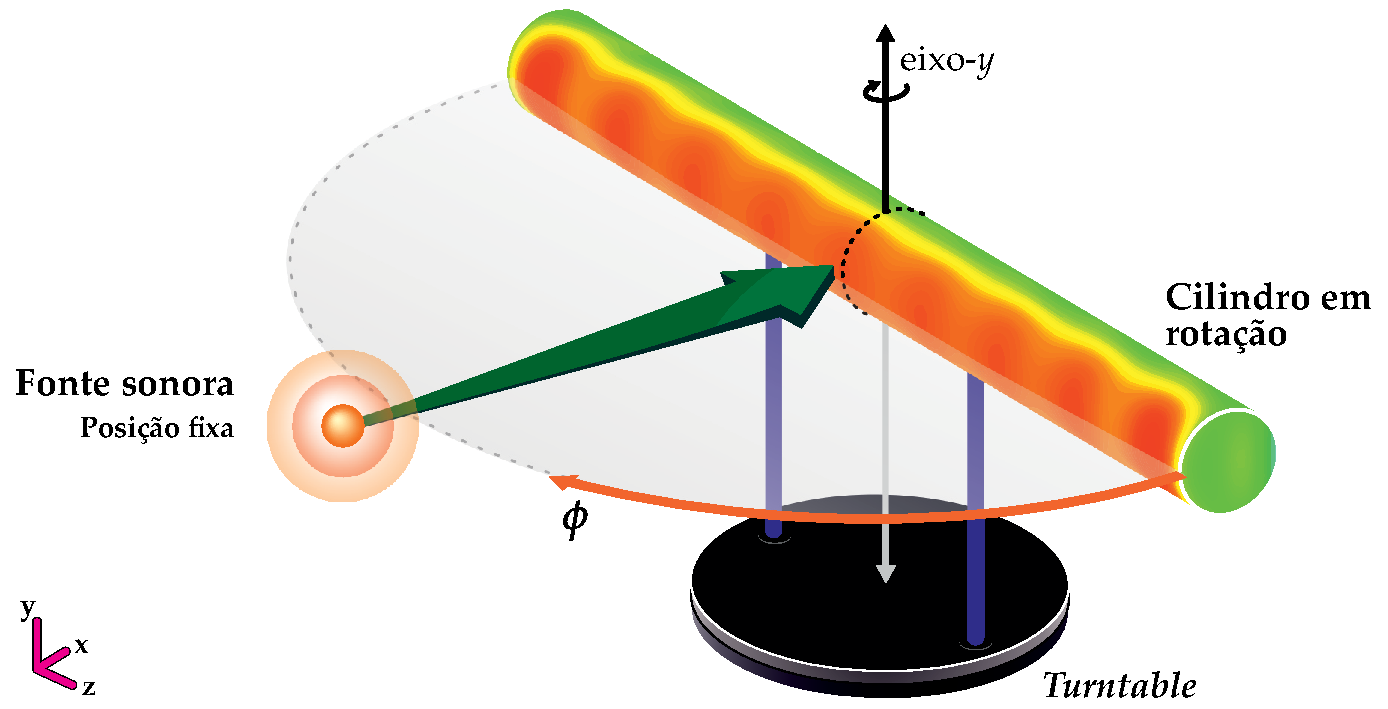
\includegraphics[width=0.74\linewidth]{Figuras/Measurement-Scheme-Fonseca-2013.pdf}%
	\caption{Medição de \textit{beamforming} com arranjo cilíndrico (adaptado de Fonseca \cite{Fonseca-2013}).\\ Exemplo de figura em duas colunas.}%
	\label{fig:beamforming}%
\end{figure*}

As figuras e tabelas devem ser inseridas durante o texto, preferencialmente em seguida aos parágrafos a que se referem. Uma menção
às figuras, tabelas, quadros e códigos no texto corrido, antes da sua apresentação, é necessária para a orientação do leitor. As figuras, tabelas e quadros devem conter todos os elementos de formatação e de conteúdo para que sejam interpretados corretamente, sem necessidade de se recorrer ao texto corrido para uma busca de informações adicionais. Deve-se separar do texto as tabelas e figuras com \textbf{1 linha} antes e depois (12~pt). 


%% Modelo de tabela em duas colunas.
\begin{table*}[!b]
  \centering \ratb{1.3} 
  \caption{Propriedades microgeométricas e macroscópicas das camadas porosas CPA 1 e CAUQ-B \cite{Mareze-2017}.\\ Exemplo de tabela em duas colunas.}
	\fontsize{11}{12}\selectfont 
    \begin{tabular}{C{2.8cm} | C{1.5cm} | C{1.5cm} | C{1.5cm} | C{1.5cm} | C{1.5cm} | C{1.0cm}| C{1.0cm}}
    \toprule
		\SetRowColor{LightOrange}
    \textbf{ Amostra / Parâmetro } & $L\txu{p}$ \qquad [$\upmu$\! m] & $L\txu{a}$ \qquad [$\upmu$\! m] & $D\txu{p}$ \qquad [$\upmu$\! m] & $D\txu{a}$ \qquad [$\upmu$\! m] & $\sigma$ [Ns/m\supe{4}] & {$\phi$\quad [--]} & $\alpha_{\infty}$ [--]\\
	  \midrule
		CPA 1 -  3\% &	1359,81 & 1492,51 & 2344,05 & 1425,67 &	5131 &	0,218 &	1,63\\
		\rowcolor[gray]{.95} CAUQ-B - 4,5\%	& 1598,29 &	701,24 & 2126,46 & 895,34 &	54989 &	0,070 &	2,89\\
    \bottomrule
    \end{tabular}
    \label{tab.exemplo}%
\end{table*}%

As figuras, tabelas e quadros deverão ser centralizados e numerados sequencialmente (vide exemplo nas \figuras{fig:beamforming} e \fign{fig:C80}; \tabela{tab.exemplo}; \Quadro{quad.exemplo} e \codigo{code.matlalatex}). Elas poderão ser colocadas em uma ou duas colunas dependendo de seu conteúdo. No caso de duas colunas, recomenda-se o posicionamento no topo ou na parte inferior da página. Busque utilizar figuras e gráficos em que seu conteúdo possa ser completamente compreendido. 

\begin{figure}[H]
	\centering \vspace{-3mm}
        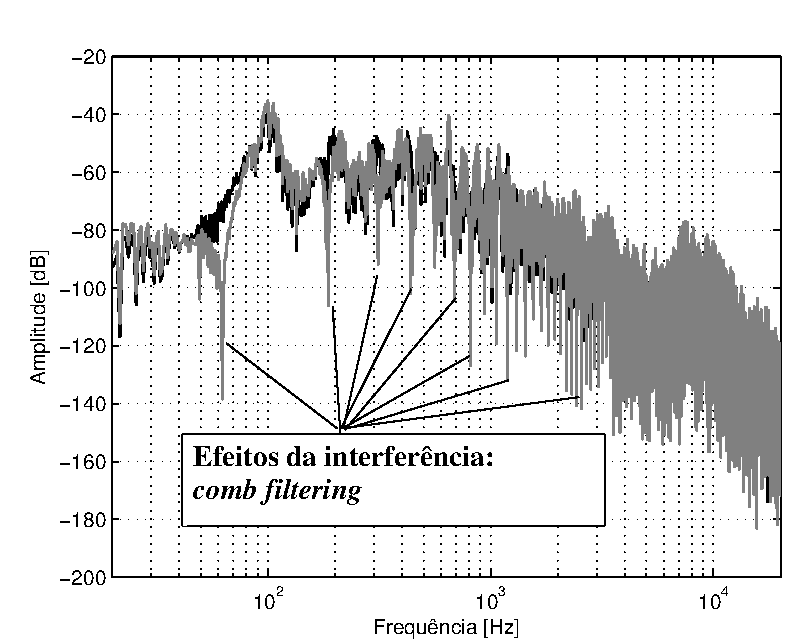
\includegraphics[width=0.96\linewidth,page=1]{Figuras/Combfilter-Brandao-2017.pdf}
        \caption{$C_{80}$ para salas distintas. As figuras podem ser colocadas lado a lado (retirado de Brandão \cite{Brandao-2017}).}
	\label{fig:C80}%
\end{figure}

\begin{quadro}[H]
%\vspace{-2mm}
  \centering \ratb{1.3} \setlength\aboverulesep{0pt} \setlength\belowrulesep{0pt}
  \caption{Este é um exemplo de um quadro.}
	\fontsize{11}{12}\selectfont 
    \begin{tabular}{| C{2.8cm} | C{1.8cm} | C{1.8cm} |}
    \hline
		\SetRowColor{LightBlue}
    \textbf{ Experimento / Tipo } & \textbf{Exp. 1} & \textbf{Exp. 2}\\
	  \midrule
		Tipo 1& Verde & Amarela\\
		\rowcolor[gray]{.95} Tipo 2 & Azul & Branco\\
    %\bottomrule
		\hline
    \end{tabular}
    \label{quad.exemplo}%
		\vspace{-0.5mm}
\end{quadro}%


%
\vspace{-3mm}
O rótulo e número das figuras, seguido da legenda, deve aparecer logo abaixo e centralizado (10~pt). Caso utilize figuras de outros autores (ou fontes), mesmo que adaptadas, indique a fonte logo após a legenda descritiva, vide exemplo da \figura{fig:beamforming}.

O rótulo, número e legenda das tabelas (quadros e códigos também) devem aparecer centralizados na parte superior (vide \tabela{tab.exemplo}). A fonte (quando necessário) das tabelas deve ser apresentada de acordo com a publicação original. A \tabela{tab.exemplo} apresenta um exemplo do estilo a ser utilizado (o conteúdo da tabela poderá conter tipografia menor que a do texto). Ademais, recomenda-se fortemente o sistema de referências cruzadas automatizado. Lembre-se que todos os objetos, como figuras e tabelas, devem ser citados no texto.
%

%


%%% Modelo de figuras lado a lado usando minipage
%\begin{figure*}[b]
    %\centering
    %\begin{minipage}[t]{.48\textwidth}
        %\centering
        %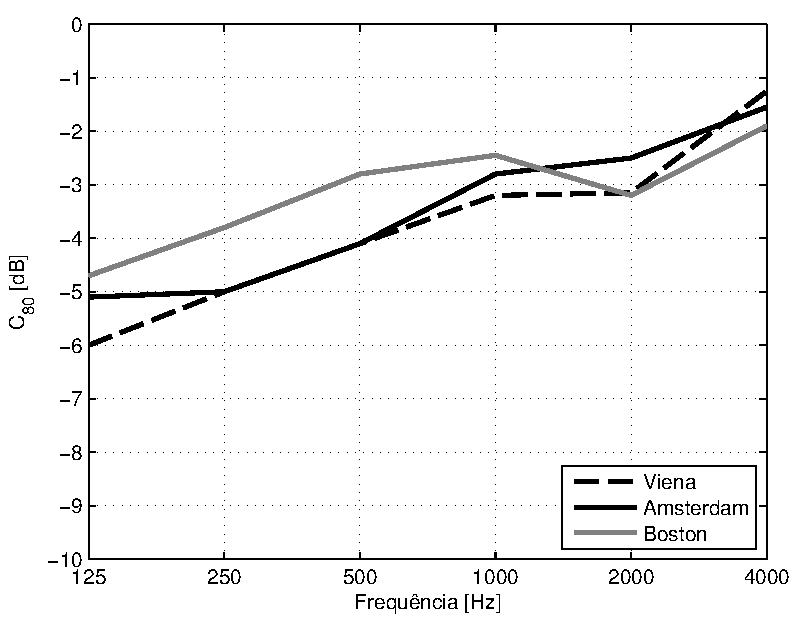
\includegraphics[width=1\linewidth,page=1]{figuras/C80_Concerthalls-Brandao-2017.pdf}
        %\caption{Efeitos de interferência em salas\\ (\textit{comb filtering}, retirado de Brandão \cite{Brandao-2017}).
%}
        %\label{fig:ladoE}
    %\end{minipage}%
		%\quad
    %\begin{minipage}[t]{0.48\textwidth}
        %\centering
        %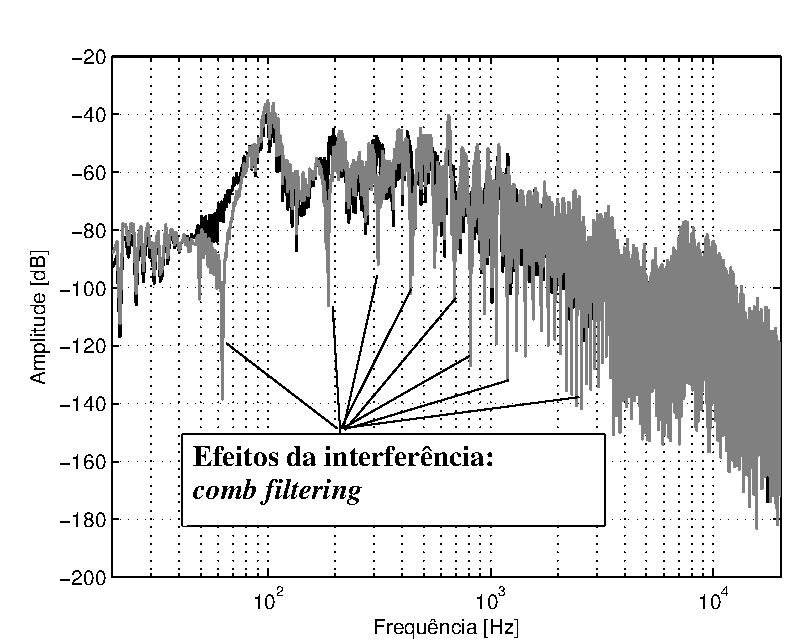
\includegraphics[width=1\linewidth,page=1]{figuras/Combfilter-Brandao-2017.pdf}
        %\caption{C$_{80}$ para salas distintas. As figuras podem ser colocadas lado a lado (retirado de Brandão \cite{Brandao-2017}).}
        %\label{fig:ladoD}
    %\end{minipage}
%\end{figure*}

Recomenda-se que gráficos, figuras, fotos e qualquer arquivo gráfico, estejam inseridos no texto em formato .jpg e/ou .png com boa qualidade (ou ainda em formato vetorial em .pdf para usuários do \LaTeX\xspace). Atente para que os elementos de gráficos e figuras sejam legíveis (sobretudo se a informação for pertinente).

A distribuição deste \textit{template} de \LaTeX\xspace inclui o pacote \ttc{Codes2Latex.sty}\footnote{Para mais detalhes consulte o arquivo \ttc{sty}.}, que habilita possibilidades para documentação de códigos genéricos e nas linguagens Matlab, Fortran, Python, LabView e Latex de forma organizada (observe o \codigo{code.matlalatex}).
%
\nomenclature[P]{Matlab}{Matrix Laboratory}

\begin{matlabcode}[Fazendo o Matlab escrever Latex (exemplo).]{code.matlalatex}
  syms x
  f = taylor(log(1+x));
  latex(f)
\end{matlabcode}

Todos os elementos podem ser coloridos ou em tons de cinza. Evite a utilização de elementos textuais de outros autores sem a devida citação (e/ou autorização). É essencial que as figuras que apresentarem texto estejam na mesma língua do artigo. Não serão aceitas citações indiretas como \textit{Google imagens}, por exemplo, assim como recomenda-se evitar o uso de bases de conhecimento voláteis como o Wikipedia.

As referências cruzadas devem ser feitas para todos os elementos, por exemplo: \figura{fig:beamforming} e \tabela{tab.exemplo} (apenas a primeira letra maiúscula). Caso exista uma subfigura, use \figura{fig:beamforming}~(a), por exemplo.


%%%%%%%%%%%%%%%%%%%%%%%%%%%%%%%%%%%%%%%%%%%%%%%%%%%%%%%%%%%%%%%%%%%%%%%%%%%%%%%%%%%%%%%%%%%%%%%%%%%%%%%%
\section{O artigo \textit{short paper}}

O evento aceitará \textbf{submissões originais} para os \textit{short papers} (isto é, ainda não publicadas) de pesquisas científicas e aplicações de engenharia, arquitetura, áudio, física, matemática e áreas afins. 
%
Algumas sugestões de áreas para publicação são:
%	
\begin{itemize}[noitemsep,topsep=-1ex] \itemsep=1.5pt
\item[\textbullet] Acústica geral; 
\item[\textbullet] Acústica não-linear; 
\item[\textbullet] Processamento de sinais; 
\item[\textbullet] Acústica virtual e auralização; 
\item[\textbullet] Imageamento acústico (\textit{beamforming},\linebreak intensimetria, holografia); 
\item[\textbullet] Acústica ambiental; 
\item[\textbullet] Acústica arquitetônica: condicionamento; 
\item[\textbullet] Acústica de edificações: isolamento; 
\item[\textbullet] Acústica fisiológica (psicoacústica), subjetiva, fonoaudiologia e saúde; 
\item[\textbullet] Métodos numéricos em acústica, vibrações e áudio;  
\item[\textbullet] Acústica subaquática e geofísica; 
\item[\textbullet] Processamento e síntese de fala; 
\item[\textbullet] Vibrações e vibroacústica;
\item[\textbullet] Acústica musical e instrumentos musicais; 
\item[\textbullet] Circuitos e dispositivos para acústica, vibrações e áudio;
\item[\textbullet] Acústica veicular e da mobilidade (automotiva, aeronáutica, ferroviária \etc); 
\item[\textbullet] Aeroacústica; 
\item[\textbullet] Bioacústica; 
\item[\textbullet] Controle de ruído; 
\item[\textbullet] Acústica industrial; 
\item[\textbullet] Áudio e eletroacústica; 
\item[\textbullet] Instrumentação e metrologia; 
\item[\textbullet] História da acústica; 
\item[\textbullet] Legislação, ética e normas;
\item[\textbullet] Ensino em acústica, vibrações e áudio;
\item[\textbullet] entre outros.
\end{itemize}
\vspace{2mm}	

%%%%%%%%%%%%%%%%%%%%%%%%%%%%%%%%%%%%%%%%%%%%%%%%%%%%%%%%%%%%%%%%%%%%%%%%%%%%%%%%%%%%%%%%%%%%%%%%%%%%%%%%
%%%%%%%%%%%%%%%%%%%%%%%%%%%%%%%%%%%%%%%%%%%%%%%%%%%%%%%%%%%%%%%%%%%%%%%%%%%%%%%%%%%%%%%%%%%%%%%%%%%%%%%%
%\section{Organização do trabalho}

A estrutura do artigo deverá contemplar pelo menos os seguintes itens (de forma breve):
Introdução; Fundamentos e/ou metodologia e/ou desenvolvimento; Resultados e discussões; Agradecimentos (opcional); e Referências. Não necessariamente existindo seções com estes nomes. 
%
%\begin{itemize}[noitemsep,topsep=0ex] \itemsep=6pt
	%\item Introdução: visão geral sobre o assunto com definição dos objetivos do trabalho, indicando a sua relevância.
	%\item Fundamentos e/ou metodologia: explorar fundamentos e métodos aplicados; 
	%\item Desenvolvimento: como o trabalho foi realizado, incluindo detalhes de teoria, materiais e métodos empregados;
	%\item Resultados e discussões: parciais ou conclusivos, conforme a modalidade do trabalho, fazendo referência a medições e cálculos estatísticos aplicados, se for o caso;
	%\item Conclusões ou Considerações finais: basear-se nas discussões e objetivos, apresentando apontamentos e considerações que findam o estudo/aplicação;
	%\item Agradecimentos: opcional, quando for pertinente;
	%\item Referências: apresentar bibliografia citada no texto.
%\end{itemize}
%


%%%%%%%%%%%%%%%%%%%%%%%%%%%%%%%%%%%%%%%%%%%%%%%%%%%%%%%%%%%%%%%%%%%%%%%%%%%%%%%%%%%%%%%%%%%%%%%%%%%%%%%%
\subsection{Citações e referências}

Para a confecção das referências deve-se utilizar a norma brasileira vigente (ABNT). As referências devem ser numeradas conforme ordem de aparição, utilizando colchetes \cite{Mareze-2019} (conforme a norma brasileira permite). Todas referências devem ser citadas durante o texto. As referências \cite{Mareze-2017,Fonseca-2013,Brandao-2017,Oppenheim-2010,Muller-2001,Mareze-2019,Borges-2018,Ristow-2016} deste modelo de artigo são apenas ilustrativas (para efeito de compreensão).
%
\nomenclature[P]{ABNT}{Associação Brasileira de Normas Técnicas}

Ao final do documento a seção de referências deve ser colocada. As entradas nela contidas devem ter tipografia com tamanho 10~pt, espaçamento simples e espaçamento de parágrafo de 8~pt. Este \textit{template} de \LaTeX\xspace usa o pacote {\ttfamily abntex2cite} que as coloca no formato correto. Recomenda-se a utilização de gerenciadores de banco de dados de bibliografia como o \href{http://www.jabref.org/}{JabRef}, \href{http://www.mendeley.com}{Mendeley} e \href{https://www.zotero.org/}{Zotero}. Em especial para usuários do Word, o Mendeley tem um \textit{plugin} para formatar e inserir as referências no documento .docx.


Dependendo do contexto, o nome do autor pode ou não ser escrito, conforme os exemplos a seguir: 
%
\begin{itemize}[noitemsep,topsep=0ex] \itemsep=4pt
	\item 	``... Mareze et al. \cite{Mareze-2019} trabalharam com absorção de materiais porosos...'' ou 
	
	\item ``... para o estudo de acústica de salas \cite{Brandao-2017} recomenda-se a leitura de um livro texto...'' ou
	\item ``... aplicando a Transformada de Fourier nos sinais de entrada \cite{Oppenheim-2010}. '' ou ainda
	\item ``... Fonseca (2013) demonstrou o cálculo de difração para superfícies cilíndricas \cite{Fonseca-2013}''.
\end{itemize}
%
Todos os autores que constam nas referências devem estar citados no texto.

Em referências com até três autores, por exemplo, Müller e Massarani \cite{Muller-2001}, ambos devem ser citados (quando evocados). No caso de mais de três autores, por exemplo, Mareze \etal \cite{Mareze-2019} deve-se citar somente o último nome do primeiro autor seguido da expressão ``\etal''. Ainda, ao citar mais de uma referência, utilize apenas um colchete, veja alguns exemplos a seguir:
%
\begin{itemize}[noitemsep,topsep=0ex] \itemsep=8pt
	\item 	``Trabalhos em temas de acústica e vibrações \cite{Mareze-2017,Fonseca-2013,Brandao-2017}.''
	\item 	``Trabalhos em temas de acústica e vibrações [\citeonline{Fonseca-2013}, \citeonline{Mareze-2017}, \citeonline{Brandao-2017}].''
	\item ``Trabalhos em temas de acústica  e áudio \cite{Mareze-2017,Oppenheim-2010,Muller-2001,Mareze-2019}.''
	\item ``Trabalhos com análise estatística aplicada \cite{Mareze-2017, Brandao-2017, Borges-2018}.''
		\item \textbf{Não usar esse estilo} ``Trabalhos com análise estatística \cite{Mareze-2017}, \cite{Brandao-2017}, \cite{Ristow-2016} ou \cite{Mareze-2017}--\cite{Ristow-2016}.''
\end{itemize}
%
Recomenda-se que as referências sejam ordenadas e compactadas (com meia-risca) como em \cite{Mareze-2017,Oppenheim-2010,Muller-2001,Mareze-2019}.

Na seção de referências, sempre que possível, inclua o ISBN, ISSN, DOI\footnote{Para usuários de Latex basta usar o campo ``doi'' de seu \texttt{.bib}.} (com link) e/ou link com a direção online em que o documento citado está disponível.

%%%%%%%%%%%%%%%%%%%%%%%%%%%%%%%%%%%%%%%%%%%%%%%%%%%%%%%%%%%%%%%%%%%%%%%%%%%%%%%%%%%%%%%%%%%%%%%%%%%%%%%%
\section{Submissão}

É responsabilidade dos autores a preparação e envio dos artigos em seu formato final. Por esse motivo, \textbf{pede-se que verifiquem com atenção a formatação de seus artigos}, especialmente gráficos e fotos, quanto à legibilidade e qualidade digital (e para impressão). Os artigos deverão ser enviados (submetidos) por e-mail nos formatos descrito a seguir:
%
%
\begin{itemize}[noitemsep,topsep=0ex] \itemsep=5pt
	\item para usuários do \textbf{Word}: .docx e .pdf com identificação; e
	\item para usuários do \textbf{\LaTeX}\xspace: .zip (contendo todo o projeto) e .pdf com identificação.
\end{itemize}

Não haverão pareceristas e/ou revisores, o conteúdo e qualidade é de inteira responsabilidade dos autores.
%
\textbf{A entrega do documento final está marcada para dia 29 de outubro de 2021.}
%\begin{itemize}[noitemsep,topsep=0ex] \itemsep=8pt
	%\item \textbf{A entrega do documento final está marcada para dia 29 de outubro de 2021.}
%\end{itemize}
%
 Será depois do evento (24 e 25 de setembro de 2021), para que autores possam coletar comentários durante a apresentação, e, com isso, ajustar detalhes para o documento final. Apenas serão rejeitados (pela comissão científica) trabalhos que apresentarem problemas graves, erros aberrantes, plágio ou outras situações não previstas.

Pelo menos um dos autores do artigo deve estar inscrito e apresentar o trabalho \textit{virtualmente} no evento.

%%%%%%%%%%%%%%%%%%%%%%%%%%%%%%%%%%%%%%%%%%%%%%%%%%%%%%%%%%%%%%%%%%%%%%%%%%%%%%%%%%%%%%%%%%%%%%%%%%%%%%%%%%%%%%%%%%%%%%%%%%%%%%%%%%%%%%%%%%%%%%%%%%%%%%%%%%%%%%%%%%%%%%%%%%%%%%%%%%%%%%%%%%
\section{Modelos para Word e \LaTeX}
O modelo de \LaTeX\xspace (.tex) foi escrito em codificação UTF8, assim é compatível com Windows, Mac, Linux e \href{https://www.overleaf.com/read/gtxwpfrgdtgk}{Overleaf}\footnote{\url{https://www.overleaf.com/read/gtxwpfrgdtgk}.}. Pode ser usado livremente para a elaboração dos artigos.
%
\nomenclature[P]{UTF8}{8-bit Unicode Transformation Format}

O modelo de .docx foi criado em Microsoft Word 2016 e, com isso, suas funcionalidades de espaçamento e configurações são garantidas para essa versão.

O autor deste texto e dos modelos/\textit{templates} é o professor William D'Andrea Fonseca, da Engenharia Acústica da Universidade Federal de Santa Maria. 

%%%%%%%%%%%%%%%%%%%%%%%%%%%%%%%%%%%%%%%%%%%%%%%%%%%%%%%%%%%%%%%%%%%%%%%%%%%%%%%%%%%%%%%%%%%%%%%%%%%%%%%%%%%%%%%%%%%%%%%%%%%%%%%%%%%%%%%%%%%%%%%%%%%%%%%%%%%%%%%%%%%%%%%%%%%%%%%%%%%%%%%%%%
\section{Considerações finais}

Buscou-se, por meio desse artigo modelo, elencar e aclarar as instruções para submissão de artigos para VI~SeGAV-e. Este próprio documento pode ser usado como modelo apenas trocando o conteúdo.

Embora esse modelo tenha 8 páginas (para poder contemplar todas as recomendações e instruções), o documento a ser entregue deve ter no máximo 6 (seis) páginas.
%
Observe o diagrama da \figura{fig:reusmao}, que contém um sumário de datas, direções do evento e informações sobre a publicação.

Em caso de dúvidas, entre em contato com a comissão científica do evento. Esperamos sua submissão e participação.


%%%%%%%%%%%%%%%%%%%%%%%%%%%%%%%%%%%%%%%%%%%%%%%%%%%%%%%%%%%%%%%%%%%%%%%%%%%%%%%%%%%%%%%%%%%%%%%%%%%%%%%%%%%%%%%%%%%%%%%%%%%%%%%%%%%%%%%%%%%%%%%%%%%%%%%%%%%%%%%%%%%%%%%%%%%%%%%%%%%%%%%%%%
\section{Agradecimentos}

Se for pertinente, faça agradecimentos.
%
Em caso de trabalhos com fomento, utilize esta seção para elucidar detalhes.

% EOF %%%%%%%%%%%%%%%%%%%%%%%%%%%%%%%%%%%%%%%%%%%%%%%%%%%%%%%%%%%%%%%%%%%%%%%%%%%%%%%%%%%%%%